\documentclass[10pt,a4paper]{ctexart}

% Compile with XeLaTeX.  Compact three-column layout; base font remains 10pt.
\usepackage[a4paper,margin=0.30in,includeheadfoot]{geometry}
\usepackage{amsmath,amssymb,mathtools}
\usepackage{graphicx}
\usepackage{siunitx}
\usepackage{multicol}
\usepackage{booktabs,tabularx,array}
\usepackage{enumitem}
\usepackage{titlesec}
\usepackage{xcolor}
\usepackage{microtype}
\usepackage{fancyhdr}
\usepackage[hidelinks]{hyperref}

\pagestyle{fancy}
\fancyhf{}
\fancyfoot[C]{\small\thepage}
\setlength{\headheight}{5pt}
\setlength{\headsep}{2pt}
\setlength{\footskip}{12pt}
\setlength{\columnsep}{0.14in}
\setlength{\columnseprule}{0.2pt}
\setlength{\parindent}{0pt}
\setlength{\parskip}{0.5pt}
\linespread{0.91}
\emergencystretch=2em

\AtBeginDocument{\fontsize{10pt}{9.1pt}\selectfont}

% Keep every text layer at or below the 10pt body size.
\titleformat{\section}{\normalsize\bfseries\color{blue!55!black}}{}{0pt}{}
\titlespacing*{\section}{0pt}{2pt}{0.5pt}
\titleformat{\subsection}{\normalsize\bfseries\color{black!75}}{}{0pt}{}
\titlespacing*{\subsection}{0pt}{1.5pt}{0pt}
\titleformat{\subsubsection}{\small\bfseries}{}{0pt}{}
\titlespacing*{\subsubsection}{0pt}{1pt}{0pt}
\setlist{nosep,leftmargin=*,topsep=0.5pt,partopsep=0pt}
\setlist[itemize]{label=\textbullet}
\setlist[enumerate]{label=\arabic*.,labelsep=0.3em}

\newcommand{\key}[1]{\textbf{#1}}
\newcommand{\bunit}[1]{\,\mathrm{#1}}
\newcommand{\formula}[1]{%
  \par\vspace{1pt}%
  \begingroup
  \setlength{\abovedisplayskip}{0pt}%
  \setlength{\belowdisplayskip}{0pt}%
  \[
    #1
  \]
  \endgroup
  \vspace{1pt}%
}
\newcolumntype{Y}{>{\raggedright\arraybackslash}X}

\begin{document}
\begin{multicols*}{3}
\sloppy


\section{1. Measurement System}
\subsection{Truthworthy chain}
\begin{itemize}
    \item  accuracy, power/portablity, calibration burden, safety/usability
\end{itemize}

\subsection{Measurand}
\begin{itemize}
    \item what exactly are we measuring, the physical quantity, property, 
    or condition the system measures.
    \item \key{Common Catagories:} biopotential, pressure, flow, imaging/dimensions, displacement, impedance, 
    temperature, chemical concentration
\end{itemize}

\subsection{Measurand chain}
\begin{itemize}
    \item measurand $\rightarrow$ transduction $\rightarrow$ conditioning $\rightarrow$ integration $\rightarrow$ performance $\rightarrow$ safety
\end{itemize}

\subsection{Convert chain}
\begin{itemize}
  \item \key{Transductor:} Converts one form of energy to another.
  \item \key{Sensor:} A transducer that converts a physical measurand to an electrical output. (Ideally responds to the measurand)
  \item \key{Convert Chain:} Measurand $\rightarrow$ Primary sensing element 
  $\rightarrow$ variable-conversion element $\rightarrow$ electrical signal.
\end{itemize}

\subsection{Conditioning}
\begin{itemize}
  \item \key{Raw signal:} small + noisy.
  \item \key{Amplify:} make it usable. 
  \item \key{Filter:} reduce unwanted content.
  \item \key{Match/isolate:} interface safely. 
  \item \key{Digitize:} prepare for processing.
  \item \key{Display:} waveform or number. \\
  The same chain applies to ECG, pulse oximetry, temperature, pressure, and other instruments.
\end{itemize}

\subsection{Generalized System}
\begin{itemize}
    \item \key{Measurand:} calibration
    \item \key{Sensor/Transducer:} feedback/ control
    \item \key{Signal Conditioning:} storage
    \item \key{Output/Display:} transmission
\end{itemize}

\subsection{Why biomedical measurement is hard}
\begin{itemize}
  \item Signals are often $\mu$V--mV, slow, and close to DC.
  \item The measurand may be inside the body or hard to isolate; patient,
  posture, motion, and time create biological variability.
  \item \key{Interfering input:} unwanted input, e.g.\ 50/60 Hz mains field.
  \item \key{Modifying input:} changes the measurement system, e.g.\ cable
  orientation or electrode--skin impedance changing mains coupling.
\end{itemize}

\subsection{Typical measurands}
\begin{center}\small
\begin{tabularx}{\linewidth}{@{}lYY@{}}
\toprule
Measurand & Typical range & Frequency range\\
\midrule
ECG & 0.5--4 mV & 0.01--250 Hz\\
EEG & $5$--$300~\mu\mathrm V$ & dc--150 Hz\\
Arterial BP (direct) & 10--400 mmHg & dc--50 Hz\\
Respiratory rate & 2--50 breaths/min & 0.1--10 Hz\\
Body temperature & $32$--$40~^\circ\mathrm C$ & dc--0.1 Hz\\
\bottomrule
\end{tabularx}
\end{center}

\subsection{Eg: Pulse oximeter chain}
\begin{itemize}
  \item Measurand: arterial oxygen saturation (SpO$_2$), inferred at the fingertip.
  \item Red + infrared light through tissue $\rightarrow$ photodetector current
  $\rightarrow$ amplify/filter/isolate the pulsatile component $\rightarrow$
  compute SpO$_2$ from a two-wavelength ratio.
  \item Performance limits: motion artifact and low perfusion.
\end{itemize}


\section{2. Static Characteristics}
\subsection{Accuracy and precision}
\begin{itemize}
  \item \key{Accuracy:} closeness to the true value.
  \item $\pm\%$ of \key{full scale}: fixed absolute error across the range.\par
    BP range 0--300 mmHg, $\pm1\%$ full scale $\Rightarrow \pm3$ mmHg.
  \item $\pm\%$ of \key{reading}: error grows with the reading.\par
    Pulse oximeter $\pm2\%$ reading: at 100\%, $\pm2\%$; at 50\%, $\pm1\%$.
  \item \key{Precision:} repeatability; high precision does not imply high accuracy.
  \item \key{Repeatability:} same conditions, same short time window.
  \item \key{Reproducibility:} conditions vary (operator, time, instrument).
\end{itemize}

\subsection{Range, span, sensitivity}
\begin{itemize}
  \item \key{Tolerance:} maximum deviation of a manufactured component from a standard value.
  \item \key{Range/span:} the minimum-to-maximum designed input values.
  \item \key{Sensitivity:} slope of the calibration line:
  \formula{\displaystyle S=\frac{\Delta\text{output}}{\Delta\text{input}}}
  Example: $\frac{\Delta R}{\Delta T}=\frac{7~\Omega}{30^\circ\mathrm C}=0.233~\Omega/^\circ\mathrm C$.
\end{itemize}

\subsection{Linearity, threshold, resolution}
\begin{itemize}
  \item \key{Linear:} if $y_1$ responds to $x_1$ and $y_2$ to $x_2$, then
  $y_1+y_2$ responds to $x_1+x_2$, and $Ky_1$ responds to $Kx_1$.
  \item \key{Independent nonlinearity:} maximum deviation from the least-squares line,
  reported as $\pm A\%$ of reading or $\pm B\%$ of full scale, whichever is larger.
  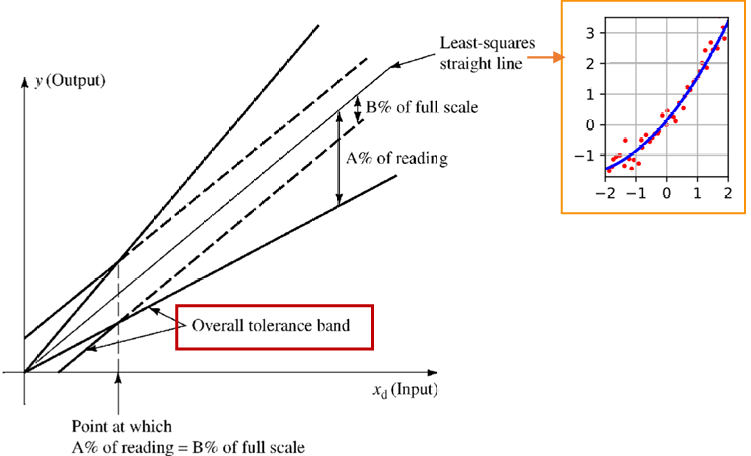
\includegraphics[width=1\linewidth]{non_linearity.png}
  \item \key{Threshold:} minimum input needed to register any output.
  \item \key{Resolution:} smallest detectable change once the instrument is moving.
\end{itemize}

\subsection{Drift, hysteresis, dead space}
\begin{itemize}
  \item \key{Zero drift} $\Delta b$: every output changes by the same absolute
  amount; slope is unchanged.
  \item \key{Sensitivity drift} $\Delta m$: slope changes; error is proportional
  to input magnitude.
  \item \key{Hysteresis:} loading and unloading curves do not coincide.
  Maximum input/output hysteresis is normally expressed as a percentage of
  full-scale input/output.
  \item \key{Dead space:} range of input values over which output does not change.
\end{itemize}


\section{3. Error, Statistics, Calibration}
\subsection{Systematic versus random error}
\begin{itemize}
  \item \key{Systematic:} consistently on one side of truth; caused by loading,
  environmental/modifying inputs, wear, or uncalibrated instruments;
  calibration or correction can fix it; averaging does not.
  \item \key{Random:} scatters unpredictably about truth; averaging reduces,
  but never eliminates, it.
  \item Mean: arithmetic average. Median: middle value after sorting. Standard deviation: spread of values about the mean.
\end{itemize}

\formula{\displaystyle
  \bar{x}=\frac{1}{n}\sum_i x_i,\qquad
  \sigma=\sqrt{\frac{\sum_i(x_i-\bar{x})^2}{n-1}}}

\begin{itemize}
  \item Gaussian distribution probability density function
  \formula{\displaystyle f(x)=\frac{1}{\sigma\sqrt{2\pi}}
  \exp\Big[-\frac{(x-\bar{x})^2}{2\sigma^2}\Big]}
  \item Gaussian rule: 68\% within $\pm\sigma$; 95.4\% within $\pm2\sigma$;
  99.7\% within $\pm3\sigma$.
\end{itemize}


\subsection{Loading effect}
\begin{itemize}
  \item A voltmeter loads a source with finite Thévenin resistance.
  \item $R_\mathrm{source}=500~\Omega$, $R_\mathrm{meter}=9500~\Omega$:
\end{itemize}

\formula{\displaystyle
  \text{loading error}=
  \frac{R_\mathrm{source}}{R_\mathrm{source}+R_\mathrm{meter}}
  =5\%}

\subsection{Uncertainty}
\begin{itemize}
  \item Independent random uncertainties combine by quadrature addition.
\end{itemize}

\formula{\displaystyle
  \begin{aligned}
    e&=\sqrt{x^2+y^2},\\
    e_\mathrm{fractional}&=\sqrt{e_1^2+e_2^2+\cdots}
  \end{aligned}}

\begin{itemize}
  \item e.g. Sensor $\pm2\%$ and amplifier $\pm1.5\%$:
  $\sqrt{0.02^2+0.015^2}=\pm2.5\%$.
\end{itemize}

\subsection{Calibration}
\begin{itemize}
  \item Use a known input and compare the instrument output with the reference.
  \item bias exists $\rightarrow$ compare to reference 
  $\rightarrow$ calibrate/correct $\rightarrow$ reference itself traceable
  \item Drift is exactly why calibration has to be repeated, not done once.
\end{itemize}


\section{4. Dynamic Characteristics}
\subsection{Common systems}
\begin{itemize}
  \item \key{Zero-order:} potentiometer, ruler
  \item \key{First-order:} thermometer, thermocouple
  \item \key{Second-order:} catherter-transducer system, acclelerometer
\end{itemize}

\subsection{First-order response}
\begin{itemize}
    \item First-order system canonical form: $\tau\frac{dy(t)}{dt}+y(t)=kx(t)$, 
    which  transfer function $\frac{Y(j\omega)}{X(j\omega)}=\frac{k}{1+j\omega\tau}$, 
    with magnitude $|H|$ and phase $\phi$.
\end{itemize}

\formula{\displaystyle
  \begin{aligned}
    |H|=\frac{k}{\sqrt{1+(\omega\tau)^2}}, \quad
    \phi=-\arctan(\omega\tau)
  \end{aligned}}

\begin{itemize}
    \item while the input is a step response $x(t)=m\cdot u(t)$, we have the output which is $y(t)=mk(1-e^{-t/\tau})$.
    \item for $t=n\tau$, the output has:0.632(n=1), 0.865(n=2), 0.950(n=3), 0.982(n=4), 0.993(n=5), 0.998(n=6), 0.9997(n=7).
\end{itemize}

\begin{itemize}
  \item $\tau$ is the time constant. Corner frequency:
  $f_c=\frac{1}{2\pi\tau}$.
  \item For $\tau=20$ ms and amplitude error under 5\%:
  $\omega\approx16.4$ rad/s, $f\approx2.6$ Hz, $\phi\approx-18.2^\circ$.
  \item A first-order system output can never be bigger than its input.
\end{itemize}

\subsection{Second-order response}
\begin{itemize}
    \item Second-order system canonical form:
\end{itemize}

\formula{\displaystyle
\begin{aligned}
\frac{d^2y(t)}{dt^2}+2\zeta\omega_n\frac{dy(t)}{dt}+\omega_n^2y(t)=k\omega_n^2x(t),
\end{aligned}}

\begin{itemize}
    \item which transfer function:  
\end{itemize}

\formula{\displaystyle
\begin{aligned}
\frac{Y(j\omega)}{X(j\omega)}=\frac{k\omega_n^2}{-\omega^2+j2\zeta\omega_n\omega+\omega_n^2}
\end{aligned}}

\begin{itemize}
    \item with parameters following:
\end{itemize}

\formula{\displaystyle
  \begin{aligned}
    \Lambda&=\ln\frac{y_1}{y_2},&
    \zeta&=\frac{\Lambda}{\sqrt{4\pi^2+\Lambda^2}},\\
    \omega_d&=\frac{2\pi}{T_d},&
    \omega_n&=\frac{\omega_d}{\sqrt{1-\zeta^2}}
  \end{aligned}}

\begin{itemize}
  \item $\omega_n$: undamped natural frequency; $\omega_d$: damped frequency
  observed in a ringing trace.
  \item $\zeta=1$: critically damped; $\zeta<1$: underdamped.
  Underdamped responses exaggerate peaks and ring; overdamped responses smear
  the waveform and understate it.
  \item Worked values $y_1=8$, $y_2=3$, $T_d=0.025$ s:
  $\Lambda=0.9808$, $\zeta\approx0.154$, $\omega_d\approx251$ rad/s,
  $\omega_n\approx254$ rad/s ($\approx40$ Hz).
\end{itemize}


\section{5. Physical Transducers}
\subsection{Transducer}
\begin{itemize}
    \item \key{Definition:} a kind of component that converts one form of energy to another.
    \item physical input $\rightarrow$ property changes $\rightarrow$ electrical signal $\rightarrow$ excitation/output
    \item e.g. potntiometer, move the effective length, change the output resistance.
\end{itemize}

\subsection{Resistive: strain gauge}
\begin{itemize}
  \item Stretching a wire makes it longer and thinner; its resistance rises.
\end{itemize}
\formula{\displaystyle
  G=\frac{\Delta R/R}{\Delta L/L}
  \quad\text{(gauge factor)},\quad
  \epsilon=\frac{\Delta L}{L}}
\begin{itemize}
  \item Force/pressure $\rightarrow$ small fractional $\Delta R$; small signal
  needs bridge read-out. Main limitation: temperature sensitivity.
\end{itemize}

\subsection{Inductive and LVDT}
\begin{itemize}
    \item Move a core inside a coil, the inductance changes, so we have:
\end{itemize}

\formula{\displaystyle L=n^2G\mu, (unit: Henry, H)}

\begin{itemize}
  \item $n$: turns; $G$: geometric form factor; $\mu$: magnetic permeability.
  \item LVDT uses mutual-inductance behavior. At null, secondary signals cancel;
  off null, imbalance gives displacement magnitude and direction.
  Frictionless, high resolution, robust; needs AC drive and is sensitive to stray
  magnetic materials.
\end{itemize}

\subsection{Capacitive}
\formula{\displaystyle C=\frac{\varepsilon_0\varepsilon_r A}{x}, unit: Farad, F}
\begin{itemize}
  \item Vary gap $x$, overlap area $A$, or dielectric constant $\varepsilon_r$.
  Non-contact, tiny displacement, low power; limited by stray capacitance and
  cable effects. Read out with high input impedance.
\end{itemize}

\subsection{Wheatstone bridge}
\formula{\displaystyle
  \begin{aligned}
    \frac{R_1}{R_2}=\frac{R_4}{R_3}\Rightarrow U_\mathrm{out}=0(at balance),
  \end{aligned}}

\begin{itemize}
  \item Sensor unbalances one or more arms; quarter/half/full bridge has 1/2/4 active arms.
  \item Approximate output: \\
  quarter-bridge: $\frac14(\Delta R/R_0)v_i$;\\
  half-bridge: $\frac12(\Delta R/R_0)v_i$; \\
  full-bridge: $(\Delta R/R_0)v_i$.\\
  e.g. $R_0=350~\Omega$, $v_i=5$ V, $G=2$, $\epsilon=10^{-3}$:
  $\Delta R=0.70~\Omega$; outputs are 2.50, 5.00, and 10.0 mV.
\end{itemize}

\subsection{Piezoelectric, thermal, optical}
\begin{itemize}
  \item Piezoelectric: generate charge by squeeze crystal:
  \formula{\displaystyle q=kf}\\
  fast, self-generating, wide dynamic range; high output impedance requires
  a charge amplifier; charge leaks, so it reports changing load, not a static load.
  \item \key{Thermistor:} resistance changes with temperature; sensitive and low cost, but nonlinear. \\
  Positive Temperature Coefficient (PTC) / Negative Temperature Coefficient (NTC)
  \item \key{Thermocouple:} wide temperature range; detect small signals; needs a cold-junction as reference.
  \item \key{Optical:} no electrical patient connection; ambient light, motion and calibration are limitations. 
  Used in pulse oximetry.
\end{itemize}

\subsection{Eg: Stimulator/pacemaker working principle}
\begin{itemize}
    \item \key{Sensor:} physical input $\rightarrow$ electrical signal
    \item \key{Actuator:} electrical command $\rightarrow$ physical action
    \item \key{Stimulator / pacemaker:} supply$\rightarrow$ oscillator $\rightarrow$ pulse output (3 stage of pulse generator)
    $\rightarrow$ leads $\rightarrow$ electrodes $\rightarrow$ tissue
\end{itemize}

\subsection{Eg: Actuators move air or liquid}
\begin{itemize}
    \item \key{Ventilator:} controller or assister; Positive or negative pressure; Time-, volume- or pressure-cycled.
    \item \key{Infusion pump and valve:} pump: drives the liquid; valve: opens or closes a flow path; a valve is a simple actuator\\
\end{itemize}


\section{6. Biopotentials}
\subsection{Origin}
\begin{itemize}
  \item The electrode is the transducer: it converts ionic current in tissue
  into electronic current in the lead.
  \item $K^+$ is high inside and Na$^+$ high outside. The Na/K pump maintains
  gradients; selective K$^+$ leak sets the resting voltage, leaving inside negative.
  \item Resting $v_m$ is about $-40$ to $-90$ mV inside relative to outside;
  nerve and cardiac cells typically $-70$ to $-90$ mV.
  \item Action potential: \\
  Na$^+$ channels open $\rightarrow$ depolarization;\\
  K$^+$ flows out $\rightarrow$ repolarization\\
  then brief hyperpolarization.
  \item Equilibrium electrial potential difference could be defined by following:
  \formula{\displaystyle V_{K} = -\frac{RT}{zF} \ln\frac{[K]_{in}}{[K]_{out}}}
  \item Surface biopotential is the summed extracellular field from many active
  sources, not the voltage of one cell. Synchronous, similarly oriented sources
  reinforce; asynchronous/opposed sources partly cancel.
\end{itemize}

\subsection{Fiber action potential}
\begin{itemize}
    \item \key{Volume conductor:} body tissue conducts current around active cells.
    \item \key{Moving charge separation:} A propagating action potential acts as a small current dipole and drives 
    local currents outside the fiber.
    \item \key{What the electrode sees:} A weak, attenuated projection of that field, not $v_m$ itself. Farther away
\end{itemize}

\subsection{Surface recording}
\begin{itemize}
    \item \key{A sum of fields:}  A surface recording adds the fields of many cells through conducting tissue.
    \item \key{What makes the sum large:}\\
    Synchronous, similarly oriented (in phrase) sources reinforce; \\
    Asynchronous or opposed ones(different timing) partly cancel.
    \item \key{Sets amplitude:} Mass of active tissue, distance to the electrode; Motor + sensory
\end{itemize}

\subsection{Bio-signal Basic Info}
\begin{itemize}
    \item \key{Electrocardiogram, ECG:}  coordinated heart-muscle activity, summed through the chest.\\
    P wave = atrial depolarization; \\
    QRS = ventricular depolarization;\\
    T wave = ventricular repolarization.
    \item \key{Electroencephalogram, EEG: }Excitatory Postsynaptic Potential/Inhibitory Postsynaptic Potential (EPSP/IPSP) in the cerebral cortex.\\
    Appears as microvolts due to distant sources, attenuated by skull and scalp.\\
    awake (activity): Beta(13-30Hz)\\
    awake (resting): Alpha(8-12Hz)\\
    sleep (drowsiness): Theta(4-7Hz)\\
    sleep (deepsleep): Delta(0.5-3Hz)\\
    \item \key{Electromyogram, EMG:} each active motor unit + the muscle fibers produces a brief extracellular motor-unit potential.
    As the force increases, more effort recruits more units $\rightarrow$ a dense interference pattern.\\
    Their extracellular potentials overlap and sum. At strong contraction, 
    individual units merge into a dense interference pattern.\\
    LOW EFFORT: few units $\rightarrow$ individual potentials visible\\
    MORE EFFORT: more recruitment + faster firing\\
    STRONG CONTRACTION: waveforms overlap $\rightarrow$ interference pattern\\
    VERY STRONG CONTRACTION: dense interference pattern
\end{itemize}

\subsection{Signal amplitude and bandwidth}
\begin{center}\small
\begin{tabularx}{\linewidth}{@{}lYY@{}}
\toprule
Signal & Amplitude & Frequency / method\\
\midrule
ECG & 0.5--4 mV & 0.01--250 Hz; skin electrodes\\
EEG & $5$--$300~\mu\mathrm V$ & dc--150 Hz; scalp electrodes\\
EMG & 0.1--5 mV & dc--10 kHz; needle electrodes\\
\bottomrule
\end{tabularx}
\end{center}

\begin{itemize}
  \item ECG: P wave = atrial depolarization; QRS = ventricular depolarization;
  T wave = ventricular repolarization.
  \item EMG: increasing force recruits more motor units and faster firing;
  overlapping extracellular potentials form a dense interference pattern.
  \item Same ECG, different purpose $\rightarrow$ different passband:
  monitor 0.67--40 Hz; diagnostic $\approx0.04$--150 Hz;
  surface EMG 15--500 Hz; needle EMG dc--10 kHz.
\end{itemize}


\section{7. Electrodes}
\subsection{Interface chemistry}
\begin{itemize}
  \item Current is carried by electrons in metal and ions in electrolyte.
  Oxidation releases electrons; reduction accepts electrons.
  \item Charge separation creates the half-cell potential $E_\mathrm{hc}$,
  set by electrode material, ion concentration, and temperature.
  The electrode adds interface voltage to the biological voltage.
  \item \key{Polarization:} departure of interface voltage from equilibrium when
  current flows; overpotential is the size of the voltage departure.
  \item \key{Non-polarizable:} no charge builds up, and charge crosses freely at steady DC
  (resistor-like). 
  \item \key{Perfectly non-polarizable:} reactions pass charge freely and
  voltage stays at equilibrium. Real electrodes lie between these limits.
\end{itemize}

\subsection{Ag/AgCl and equivalent circuit}
\begin{itemize}
  \item Ag/AgCl with chloride gel has stable interface potential, less baseline
  drift, and low interface impedance. It is useful because its interface stays
  stable, not because $E_\mathrm{hc}$ is small.
  \item Model: $E_\mathrm{hc}$ (battery), $C_d$ (double-layer charge storage),
  $R_d$ (leakage across double layer), $R_s$ (interface/electrolyte resistance);
  $R_d\parallel C_d$.
\end{itemize}

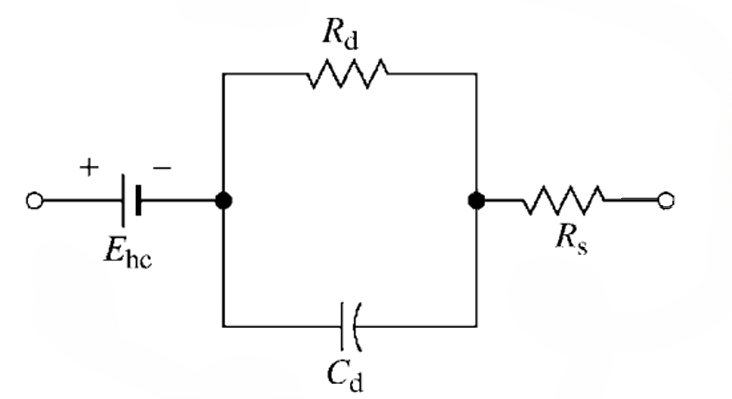
\includegraphics[width=1\linewidth]{AgCl_electricmodel.png}

\formula{\displaystyle
  \begin{aligned}
    Z_e(f)&\approx R_s+R_d &&\text{at low }f,\\
    Z_e(f)&\rightarrow R_s &&\text{at high }f
  \end{aligned}}

\begin{itemize}
  \item Electrode impedance is highest at low frequency and approaches $R_s$
  at high frequency because $C_d$ provides an easier path.
  \item A suitable AgCl coating lowers low-frequency impedance, but more coating is not always better.
\end{itemize}

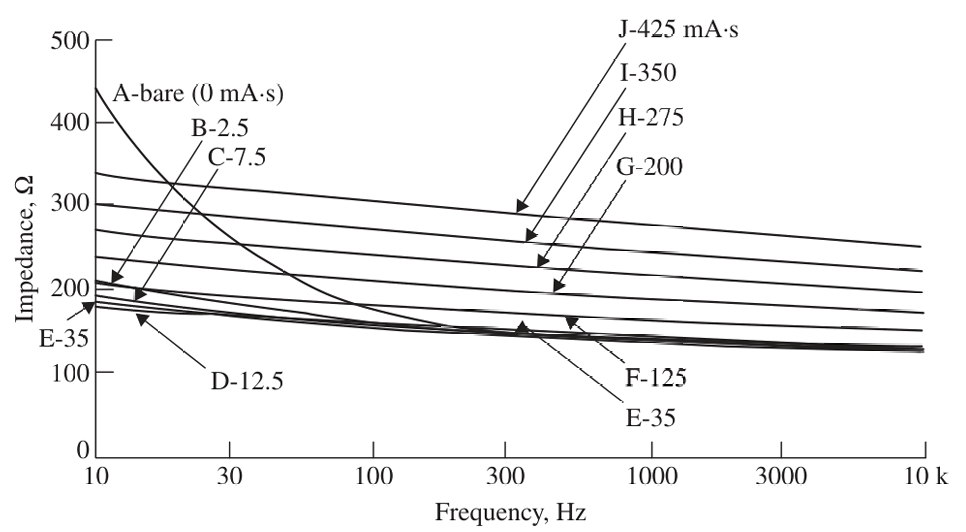
\includegraphics[width=1\linewidth]{AgCl_Imf.png}

\subsection{Skin and artifacts}
\begin{itemize}
  \item Good electrode material alone cannot guarantee good contact with the body.
  \item Electrode provides metal contact; Gel / Sweat provides ionic contact;
  Epidermis is outer skin layer; its outermost part, the stratum corneum, is the main barrier;
  Deeper tissue is dermis and below and conducts well.
  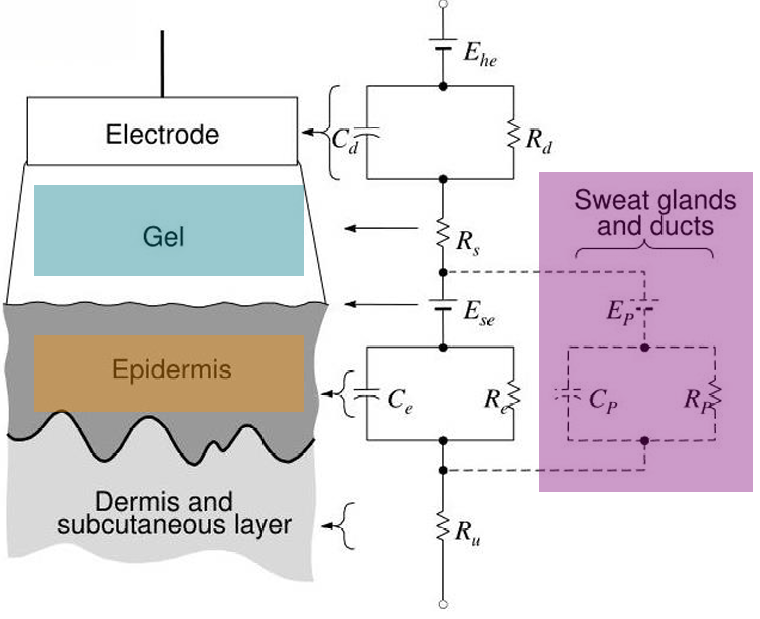
\includegraphics[width=1\linewidth]{skin_detectmodel.png}
  \item \key{Already met:} $E_{hc}, R_d, C_d, R_s$: electrode–gel interface
  \item \key{New: epidermis} $E_{se}$: gel–skin potential; $R_e ∥ C_e$: skin resistance and capacitance.
  \item $R_u$: resistance of the deeper tissue.
  \item \key{Dashed branch:} sweat glands: an extra path (set aside).
  \item Skin adds impedance and can change with sweat, pressure, hair, and motion.
  \item Movement changes the electrode--skin interface and produces baseline wander;
  a filter cannot fully remove artifact that overlaps useful signal.
  \item Stable electrodes and good skin contact reduce motion artifact, but cannot guarantee its elimination
  \item Improve contact: prepare skin, secure electrode, use balanced low impedances, and reduce cable movement.
\end{itemize}


\section{8. Amplifiers}
\subsection{Analog front end}
\begin{itemize}
  \item Circuits receive and prepare the electrode signal.
  \item \key{Read accurately:} Draw little current (high input impedance). 
  Measure the voltage difference and reduce shared interference.
  \item \key{Prepare for the ADC:} Amplify within the available range (gain).
  Keep the frequencies needed for the ECG (bandwidth).
  \item \key{Protect the patient:} Protection limits electrical hazards.
  Isolation interrupts a direct conductive path to the recorder.
  \item The electrode offset can be much larger than the ECG signal. \\
  e.g. ECG input dynamic range $\pm5$ mV; DC offset
  $\pm300$ mV; input impedance at 10 Hz $\ge2.5$ M$\Omega$ (design aim
  $\sim10$ M$\Omega$); system noise $\le30~\mu$V peak-to-peak.
\end{itemize}

\subsection{Operational amplifier}
\begin{itemize}
  \item An op amp amplifies the difference between its inputs; feedback sets a usable gain.
  \item Amplifies the difference between its two inputs by an enormous factor; 
  feedback through external resistors sets a useful, predictable gain.
  \item \key{Amp working rules:} \\
  1. When the op-amp output is in its linear range, the two input terminals are nearly equal.\\
  2. No current flows into either input terminal of the op amp.
  \item The ECG differs between the two electrodes (differential voltage $v_d$); 
  interference is nearly the same at both (common-mode voltage $v_{cm}$).
\end{itemize}

\formula{\displaystyle
  \begin{aligned}
    v_d&=v_2-v_1, \quad  v_\mathrm{cm}&=\frac{v_2+v_1}{2}
  \end{aligned}}

\begin{itemize}
    \item \key{Common mode rejection ratio (CMRR):} the ability of Op amp to amplify differential signal and reject Common Mode signal.
\end{itemize}

\formula{\displaystyle
  \begin{aligned}
    \mathrm{CMRR}=\frac{G_d}{G_c}
  \end{aligned}}

\begin{itemize}
  \item Differential signal is wanted ECG; common-mode signal is nearly equal interference on both leads. 
  A good biopotential amplifier has CMRR above 10,000.
  \item Large electrode DC offset limits gain before offset removal. For a
  0--3.3 V, 12-bit ADC and 4 mV ECG, $G_\mathrm{total}\le825$; illustrative
  headroom choice $G_\mathrm{total}\approx600$.\\
  e.g. Common-mode on the body $V_{cm} \approx 10 mV$; target $\le$ 10 $/\mu V$ referred to the input\\
   $\frac{V_{cm}}{CMRR} \le 10 \mu V\rightarrow CMRR \ge 1000$\\
   $\rightarrow 20 \cdot log_{10}(1000)= 60$ dB.
   \item At poor enviroment, $V_{cm} \approx 50 mV$, which means CMRR $\ge 5000$ or 74 dB.
\end{itemize}

\subsection{Amplifier cascade}
\begin{itemize}
  \item An op-amp senses the difference, but wired simply it drains the tiny electrode signal.
  \item A buffer copies its input voltage while drawing almost no current, so the high-resistance electrodes are barely loaded.
  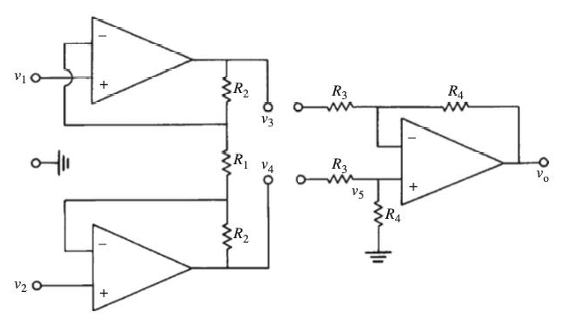
\includegraphics[width=1\linewidth]{amp_cascade.png}
  \item Why not just an op amp?\\
  A plain one-op-amp difference circuit has low input resistance; 
  skin electrodes have high, unequal resistance, so it drains and unbalances the signal, undoing the rejection we just built.
  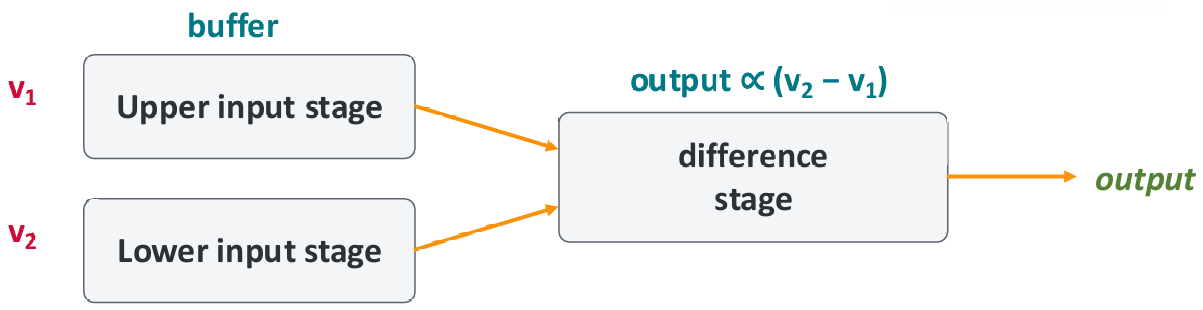
\includegraphics[width=1\linewidth]{amp_cascade_principle.png}
  The instrumentation amplifier make two input buffers give very high input impedance, 
  the difference stage rejects the shared interference, 
  and one external resistor sets the gain all in one chip (like LT1920, AD620)
\end{itemize}

\subsection{Input impedance}
\begin{itemize}
  \item Unequal electrode impedances turn common-mode voltage into a differential error.
  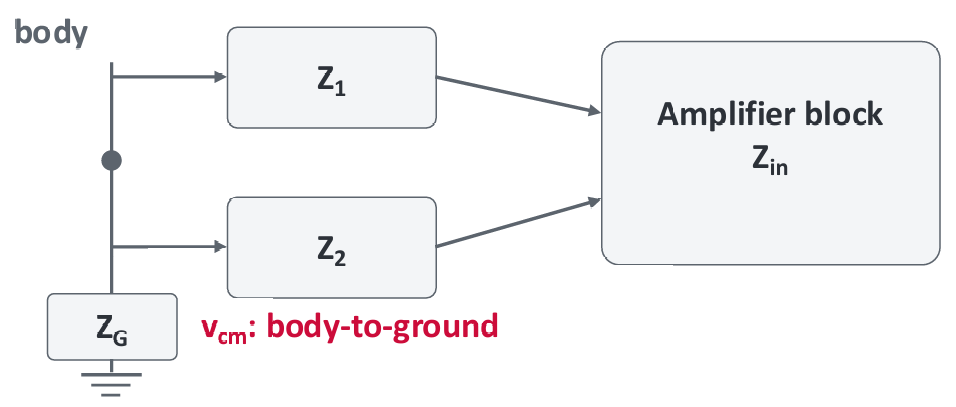
\includegraphics[width=1\linewidth]{input_impedance.png}
  \item high amplifier CMRR is not enough, unequal electrode impedances with finite $Z_{in}$ convert common-mode interference into a differential error.
  \item e.g. $V_{cm} \approx 10 mV; target \le 10 \mu V$ \\
  $Z_1 - Z_2 = 20 k\Omega, Z_{in} = 5 M\Omega$ \\
  $V_d \approx V_{cm} \cdot (\frac{Z_2 - Z_1}{Z_{in}}) \approx 40 \mu V> 10 \mu V$
  \item \key{How to design:} use high input impedance, keep the electrodes balanced, and reduce the common-mode voltage.
\end{itemize}


\section{9.Isolation and protection}
\subsection{Why needs barrier}
\begin{itemize}
  \item patient-electrodes-\textbf{BARRIER}-mainpowerinstrument-AC(220v50Hz)
  \item \key{What create risk:} electrodes make an electrical connection to the patient, 
  so a fault in the mainspowered instrument must not open a direct current path through that connection.
  \item The isolation barrier passes the measurement while interrupting a direct route for a mains-side fault current
\end{itemize}

\subsection{Where is barrier}
\begin{itemize}
  \item \key{Patient side:} protection, preamplifier, protection receives the electrode signal; 
  the preamplifier raises the small ECG.
  \item \key{ISOLATION BARRIER:} the measurement passes; references stay separate.
  \item \key{Recorder side:} driver amplifier, ADC and microcontroller, 
  the driver passes the signal to the ADC for digitizing.
  \item The recorder receives the signal across the barrier while its electrical reference stays separate.
\end{itemize}

\subsection{Barrier function}
\begin{itemize}
  \item \key{Patient side:} instrumentation amplifier $\rightarrow$ unity-gain stage own supply and ground
  \item \key{ISOLATION BARRIER}
  \item \key{Recorder side:} separate supply and ground, mains-referenced
  \item What crosses the barrier: information about the measured ECG voltage.
  \item What stays separate: the patient-side and recorder-side supplies and grounds.
  \item The signal crosses; a direct fault-current path does not.
\end{itemize}


\section{10. Filters, Noise, Interference}
\subsection{Filters}
\formula{\displaystyle
  f_c=\frac{1}{2\pi RC}=\frac{1}{2\pi\tau}}
\begin{itemize}
  \item High-pass removes electrode DC offset and slow drift:
  monitor ECG 0.67 Hz; diagnostic ECG 0.04 Hz.
  \item Low-pass limits bandwidth and cuts high-frequency corruption/anti-alias:
  monitor ECG 40 Hz; diagnostic ECG 150 Hz.
  \item Band-pass combines high-pass and low-pass. Notch removes one frequency;
  50 Hz mains notch is a last resort because 50 Hz lies inside diagnostic band.
  \item Higher high-pass corner rejects more motion artifact but distorts slow
  features; choice depends on monitor versus diagnostic purpose.
\end{itemize}

\subsection{Where corruption comes from}
\begin{itemize}
  \item \key{Intrinsic noise:} thermal and $1/f$ noise; use a low-noise first
  stage and limit bandwidth.
  \item \key{External interference:} 50 Hz mains, EMI, ground loops; shield,
  twist, ground correctly, use driven-right-leg and high input impedance.
  \item \key{Physiological/interface artifact:} EMG, motion, offset saturation;
  electrode choice/placement, skin preparation, gain staging.
\end{itemize}

\subsection{Diagnosis and mitigation}
\begin{itemize}
  \item \key{Periodic mains pickup:} periodic ripple at mains frequency $\rightarrow$ mains coupling:
  shield/twist leads, improve electrode contact, DRL; notch last.
  \item \key{Movement/interface artifact:} slow baseline wander with movement $\rightarrow$ secure interface,
  fixation/skin preparation.
  \item \key{Muscle activity or EMI:} irregular high-frequency bursts $\rightarrow$ EMG or radiated EMI:
  move off muscle or apply appropriate EMI filtering.
  \item \key{Clipping and saturation:} flattened peaks $\rightarrow$ offset $\times$ gain exceeds linear range:
  lower gain, then AC-couple.
  \item Electric-field coupling: shielded leads grounded at instrument, lower skin–electrode impedance.\\
  Common-mode on the body: high $Z_{in}$, balanced electrodes, driven-right-leg.\\
  Magnetic induction: twist wires and keep them close to body.\\
  Ground loop: one ground point for all instruments on the patient.\\
  EMI: small capacitor across the inputs; amplifiers with built-in EMI filtering
\end{itemize}

\subsection{Eg: Driven-right-leg}
\begin{itemize}
  \item Sense common-mode voltage, invert and amplify it, then feed it back to
  the right-leg electrode; feedback drives $v_\mathrm{cm}$ down.
  \item It effectively grounds the patient without a direct ground connection.
  \item e.g. 100 k$\Omega$ right-leg electrode appears as $\approx249~\Omega$;
  $v_\mathrm{cm}$ falls from 10 mV to $\approx50~\mu$V.
\end{itemize}


\section{11. Sampling and ADC}
\subsection{Sampling and aliasing}
\formula{\displaystyle f_s\ge2f_\mathrm{max}}
\begin{itemize}
  \item Sampling measures voltage at regular instants. Below Nyquist, high
  frequencies fold down into false low frequencies (aliasing).
  \item An analog anti-aliasing low-pass filter must act \key{before} the ADC.
  For monitor ECG $f_\mathrm{max}=40$ Hz $\Rightarrow f_s\ge80$ Hz;
  diagnostic $f_\mathrm{max}=150$ Hz $\Rightarrow f_s\ge300$ Hz.
  At 400 samples/s, Nyquist is 200 Hz.
\end{itemize}

\subsection{Quantization and resolution}
\formula{\displaystyle
  q=\frac{V_\mathrm{ref}}{2^{N_b}},\qquad
  e_\mathrm{max}=\frac q2}
\begin{itemize}
  \item ADC rounds input to the nearest available level. A 12-bit, 3.3 V ADC
  has 4096 codes, $q=3.3/4096\approx0.806$ mV, maximum error
  $e_{max}\approx0.403$ mV.
  \item With total gain $G\approx600$, electrode-referred step
  $q/G\approx1.34~\mu$V. A 1 mV electrode change becomes 600 mV,
  or about $600/0.806\approx745$ ADC steps.
\end{itemize}


\end{multicols*}
\end{document}
